\chapter{Extending RDF}
\label{ch7}

RDF allows us to represent data as a graph, and as we have seen in Chapter~\ref{ch5}, when we use HTTP URIs as 
identifiers in RDF, we can weave a world-wide Web of data.  This Web of data already exists and has billions of triples. The Semantic Web standards build on top of RDF to provide more modeling capabilities for the Web of data.  There are two basic ideas at play in these extensions:

\begin{itemize}
    \item \emph{Inference}, where we draw conclusions based on data we have already seen.  Inference is
    a way to create new data from existing data. 
    \item \emph{Expectation} where we form some prediction about data we haven't yet seen.  Expectation is useful when 
    eliciting data from a user or for validating data from a new data source. 
\end{itemize}

\section{Inference in RDF}



Suppose you hit the web page of an online clothing retailer, and you
search for ``chamois'' in the category of ``Shirts.'' Your search comes
up empty. You are surprised, because you were quite certain that you saw
a chamois Henley in the paper catalog that landed in your mailbox. So
you look up the unit number in the catalog and do another search, using
that. Sure enough, there is the chamois Henley. Furthermore, you find
that ``Henleys'' is shown in the catalog as a kind of ``Shirts.'' You might
mutter to yourself. ``If it comes up under `Henleys,' it should come up
under `Shirts.' What's the matter with this thing?''

What do we expect from a search like this? We want any search, query, or
other access to the data that reference ``Shirts'' to also look at
``Henleys.'' What is so special about the relationship between
``Shirts'' and ``Henleys'' to make us expect this? That is what we mean
when we say, ```Henleys' is a kind of `Shirts.' '' How can we express
this meaning in a way that is consistent and maintainable?

One solution to this problem is to leverage the power of the query;
after all, in conventional database applications, it is in the query
where relationships among data elements are elaborated. In this case, we
could use the transitive query facility in SPARQL (Chapter\ref{ch5}) to write a
query to search all of the shirts. If we represent relationships between
categories with :subClassOf, we could write:

\begin{lstlisting}
SELECT ?item
WHERE {?class :subClassOf :Shirts .
       ?item a ?class . }
\end{lstlisting}


In addition to this approach, the Semantic Web also provides a model of
data expression that allows for explicit representation of the
relationship between various data items. In this sense, it genuinely
allows a data modeler to create data that are more connected, better
integrated, and in which the consistency constraints on the data can be
expressed in the data itself. The data can describe something about the
way they should be used.

As an alternative to this approach, the Semantic Web stack includes a
series of layers on top of the RDF layer to describe consistency
constraints in the data. The key to these levels is the notion of
\emph{inferencing}. In the context of the Semantic Web, inferencing
simply means that given some stated information, we can determine other,
related information that we can also consider as if it had been stated.
In the Henleys/Shirts example, we would infer that any members of the
class ``Henleys'' is also a member of the class ``Shirts.'' Inferencing
is a powerful mechanism for dealing with information, and it can cover a
wide range of elaborate processing. For the purposes of making our data
more integrated and consistent, very simple inferences are often more
useful than elaborate ones. As a simple example, in Chapter\ref{ch6}, we saw
how to write a set of queries to maintain relationship information in a
family tree, whether the information was originally expressed about
children, brothers, sisters, mothers, sons, etc. It is this sort of
mundane consistency completion of data that can be done with inferencing
in the Semantic Web. Although inferencing of this sort seems trivial
from the point of view of the natural world (after all, doesn't everyone
just know that this is the way families work?), it is the lack of just
this sort of correlation that keeps data inconsistent and is vital to
scenarios such as the search engine we mentioned.

\subsection{Inference in the Semantic Web}

To make our data seem more connected and consistently integrated, we
must be able to add relationships into the data that will constrain how
the data are viewed. We want to be able to express the relationship
between ``Henleys'' and ``Shirts'' that will tell us that any item in
the ``Henleys'' category should also be in the ``Shirts'' category. We
want to express the fact about locations that says that if a hotel chain
has a hotel at a particular location, then that location is served by a
hotel in that chain. We want to express the list of planets in terms of
the classifications of the various bodies in the solar system.

Many of these relationships are familiar to information modelers in many
paradigms. Let's take the relationship between ``Henleys'' and
``Shirts'' as an example. Thesaurus writers are familiar with the notion
of \emph{broader term}. ``Shirts'' is a broader term than ``Henleys.''
Object-oriented programmers are accustomed to the notion of subclasses
or class extensions. ``Henleys'' is a subclass of, or extends, the class
``Shirts.'' In the RDF Schema language, to be described in Chapter~\ref{ch8}, we say, ``Henleys'' subClassOf ``Shirts.''  
In the Simple Knowledge Organization System (SKOS) which we describe in Chapter~\ref{ch11}, we say ``Shirts'' broader term ``Henleys''. 
It is all well and
good to say these things, but what do they mean?

Thesauri take an informal stance on what these things mean in a number
of contexts. If you use
a broader term in a search, you will also find all the entries that were
tagged with the narrower term. If you classify something according to a
broad term, you may be offered a list of the narrower terms to choose
from to focus your classification.

\begin{sidebar}{}
Many readers may be familiar with terms like \emph{class} and
\emph{subclass} from Object-Oriented Programming (OOP). There is a close
historical and technical relationship between the use of these and other
terms in OOP and their use in the Semantic Web, but there are also
important and subtle differences. OOP systems take a more formal, if
programmatic, view of class relationships than that taken by thesauri
and taxonomies. An object whose type is ``Henleys'' will respond to all
messages defined for object of type ``Shirts.'' Furthermore, the action
associated with this call will be the same for all ``Shirts,'' unless a
more specific behavior has been defined for ``Henley,'' and so on. The
Semantic Web also takes a formal view of these relationships, but in
contrast to the programmatic definition found in OOP, the Semantic Web
defines the meaning of these things in terms of inference.
\end{sidebar}


The Semantic Web infrastructure provides a formal and elegant
specification of the meaning of the various terms like subClassOf. For
example, the meaning of ``B is a SubClassOf C'' is ``Every member of
class B is also a member of class C.'' This specification is expressed
in the form of an inference. From the information ``x is a member of
B,'' one can derive the new information, ``x is a member of C.''

For the next several chapters, we will introduce terms that can be used
in an RDF model, along with a statement of what each term means. This
statement of meaning will be given in the form of an inference pattern:
``Given some initial information, the following new information can be
derived.'' This is how the RDF Schema language (RDFS, Chapter\ref{ch8}) and the
Web Ontology Language (OWL, Chapter\ref{ch12}) work.

Our first example is one that we can use with the Henleys and Shirts
example. The meaning for

rdfs:subClassOf is given by the following inference:

\begin{lstlisting}
IF
?A rdfs:subClassOf ?B. AND
?x rdf:type ?A. THEN
?x rdf:type ?B.
\end{lstlisting}

In plain English, this says that if one class A is a subclass of another
class B, anything of type A is also of type B. This simple statement is
the entire definition of the meaning of subClassOf in the RDF Schema
language. We will refer to this rule as the \emph{type propagation
rule}. This very simple interpretation of the subclass relationship
makes it a workhorse for RDFS modeling (and also for OWL modeling, as
described in subsequent chapters). It closely corresponds to the IF/THEN
construct of programming languages: IF something is a member of the
subclass, THEN it is a member of the superclass.

\begin{sidebar}{}
The Semantic Web definition of subClassOf is similar to the definition
of subclass or extension in OOP. In OOP, an instance of some class
responds to the same methods in the same way that instances of its
superclass do. In Semantic Web terms, this is because that instance is
also a member of the superclass, and thus must behave like any such
member. For example, the reason why an instance of class ``Henleys''
responds to methods defined in ``Shirts'' is because the instance
actually is also a member of class ``Shirts.''

This similarity only goes so far. For example, it breaks down when, in
the OOP system, the subclass defines an override for a method defined in
the superclass. In Semantic Web terms, the instances of ``Henleys'' are
still instance of ``Shirts'' and should respond accordingly. But in most
OOP semantics, this is not the case; the definitions at ``Henleys'' take
precedence over those at ``Shirts,'' and thus ``Henleys'' need not
actually behave like ``Shirts'' at all. In the logic of the Semantic
Web, this is not allowed.
\end{sidebar}

\subsection{SPARQL and inference}

Often, we can express the inference rules of RDFS (and OWL) by using
SPARQL CONSTRUCT. For example, since a CONSTRUCT query specifies new
triples based on a graph pattern of triples found in
the data, in the case of the type propagation rule, we can specify the
type propagation rule with the following SPARQL CONSTRUCT query:

\begin{lstlisting}
CONSTRUCT {?r rdf:type ?B}
WHERE { ?A rdfs:subClassOf ?B .
        ?r rdf:type ?A }
\end{lstlisting}

SPARQL provides a precise and compact way to express inference rules of
this sort. We will use this SPARQL notation throughout the rest of the
book to describe much of the inferencing in RDFS and OWL. It is a clean,
concise way to specify inferences, provide ample examples of SPARQL
queries, and show the relationship between SPARQL and these other
Semantic Web languages.

Using SPARQL to define inference isn't just a convenience for writing a
book---SPARQL can be used as the basis for an inference language itself.
One proposal for such an inference language is called SPARQL Inferencing
Notation (SPIN)\footnote{http://spinrdf.org/}. SPIN includes a number of constructs for managing
inferencing with SPARQL, but for the purposes of this book, SPIN is
simply a way to specify that a particular CONSTRUCT query is to be used
as a definition for inferences for a particular model. For example, if
we want to say that the type propagation rule holds for all members of
the class Shirt, we can specify this in SPIN as

\begin{lstlisting}
:Shirt spin:rule "CONSTRUCT {?this rdf:type ?B}
                  WHERE {?A rdfs:subClassOf ?B .
                         ?this rdf:type ?A}" .
\end{lstlisting}

The variable ?this has special meaning in SPIN; it refers to a member of
the class that the query is attached to by spin:rule. In this example,
?this refers to any member of the class :Shirt. We will use SPIN from
time to time to elaborate how inferences in RDFS and OWL are related to
constructions that can be specified in SPARQL.

\subsection{Virtues of inference-based semantics}

Inference patterns constitute an elegant way to define the meaning of a
data construct. But is this approach really useful? Why is it a
particularly effective way to define the meaning of constructs in the
Semantic Web?

Since our data are living in the Web, a major concern for making our
data more useful is to have them behave in a consistent way when
combined with data from multiple sources. The strategy of basing the
meaning of our terms on inferencing provides a robust solution to
understanding the meaning of novel combinations of terms. Taking
subClassOf as an example. It is not out of the question for a single
class to be specified as subClassOf two other classes. What does this
mean?

In an informal thesaurus setting, the meaning of such a construct is
decided informally: What do we
want such an expression to mean? Since we have a clear but informal
notion of what broader term means, we can use that intuition to argue
for a number of positions, including but not limited to, deciding that
such a situation should not be allowed, to defining search behavior for
all terms involved. When the meaning of a construct like broader term is
defined informally, the interpretation of novel combinations must be
resolved by consensus or authoritative proclamation.


\begin{sidebar}{}
OOP also faces the issue of deciding an appropriate interpretation for a
single subclass of two distinct classes. The issue is known as multiple
inheritance, and it is much discussed in OOP circles. Indeed, each OOP
modeling system has a response to this issue, ranging from a refusal to
allow it (C\#), a distinction between different types of inheritance
(interface vs. implementation inheritance, e.g., Java), to complex
systems for defining such things (e.g., the Meta-Object Protocol of the
Common Lisp Object System). Each of these provides an answer to the
multiple inheritance question, and each is responsive to particular
design considerations that are important for the respective programming
language.
\end{sidebar}

In an inference-based system like the Semantic Web, the answer to this
question (for better or worse) is defined by the interaction of the
basic inference patterns. How does multiple inheritance work in the RDF
Schema Language? Just apply the rule twice. If A is subClassOf B and A
is also subClassOf C, then any individual x that is a member of A will
also be a member of B and of C. No discussion is needed, no design
decisions. The meaning of subClassOf, in any context, is given elegant
expression in a single simple rule: the type propagation rule. This
feature of inference systems is particularly suited to a Semantic Web
context, in which novel combinations of relationships are bound to occur
as data from multiple sources are merged.

\section{Where are the Smarts?}

An inference-based system for describing the meaning of Semantic Web
constructs is elegant and useful in a distributed setting, but how does
it help us make our data more useful? For our application to behave
differently, we will need a new capability in our deployment
architecture, something that will respond to queries based not only on
the triples that have been asserted but also on the triples that can be
inferred based on the rules of inference. This architecture is shown in
Figure~\ref{fig:ch7.1}, and it is very similar to the RDF query architecture shown
in Figure~\ref{fig:ch4.4}.

\begin{figure}
\centering
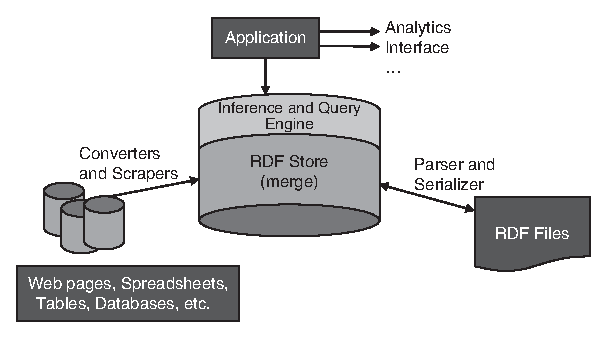
\includegraphics[width=5in]{media/ch7/f07-01.eps}
\caption{Semantic Web architecture with inferencing.}
\label{fig:ch7.1}
\end{figure}

The novelty of this architecture is an inferencing capability that
stands with the query component between the application and the RDF data
store. The power of a query engine with inferencing capability is
determined by the set of inferences that it supports. An RDFS inference
query engine supports a small set of inferences defined in the RDFS
standard; an OWL inference query engine supports the larger set of OWL
inferences. (Note that there are alternative formulations where the data
are pre-processed by an inferencing engine and then queried directly. We
discuss this later in this chapter.)

\begin{example}{Simple RDFS Query}
\label{ex:7.1}

Suppose we have an inference engine that includes support for the type
propagation rule working over an RDF
store that contains only these two triples:

\begin{lstlisting}
shop:Henleys rdfs:subClassOf shop:Shirts. 
shop:ChamoisHenley rdf:type shop:Henleys.
\end{lstlisting}

Suppose we have a SPARQL triple pattern that we use to examine these
triples, thus:

\textbf{Ask:}

\begin{lstlisting}
SELECT ?item
WHERE {?item rdf:type shop:Shirts . }
\end{lstlisting}

In a plain RDF query situation, this pattern will match no triples
because there is no triple with predicate rdf:type and object
shop:Shirts. However, since the RDFS inference standard includes the
type propagation rule just listed, with an RDFS inferencing query
engine, the following single result will be returned:

\textbf{Answer:}

\begin{tabular}{|l|}
\hline
?item\\
\hline
Shop:ChamoisHenley\\
\hline
\end{tabular}

\subsection{Asserted triples versus inferred triples}

It is often convenient to think about inferencing and queries as
separate processes, in which an inference engine produces all the
possible inferred triples, based on a particular set of inference rules.
Then, in a separate pass, an ordinary SPARQL query engine runs over the
resulting augmented triple store. It then becomes meaningful to speak of
\emph{asserted triples} versus \emph{inferred triples}.

Asserted triples, as the name suggests, are the triples that were
asserted in the original RDF store. In the case where the store was
populated by merging triples from many sources, all the triples are
asserted. Inferred triples are the additional triples that are inferred
by one of the inference rules that govern a particular inference engine.
It is, of course, possible for the inference engine to infer a triple
that has already been asserted. In this case, we still consider the
triple to have been asserted. It is important to note that there is no
logical distinction between inferred and asserted triples, the inference
engine will draw exactly the same conclusions from an inferred triple as
it would have done, had that same triple been asserted.
\end{example}

\begin{example}{Asserted versus Inferred Triples}

Even with a single inference rule like the type propagation rule, we can
show the distinction of asserted vs. inferred triples. Suppose we have
the following triples in a triple store:

\begin{lstlisting}
shop:Henleys rdfs:subClassOf shop:Shirts. 
shop:Shirts rdfs:subClassOf shop:MensWear. 
shop:Blouses rdfs:subClassOf shop:WomensWear.
shop:Oxfords rdfs:subClassOf shop:Shirts. 
shop:Tshirts rdfs:subClassOf shop:Shirts. 
shop:ChamoisHenley rdf:type shop:Henleys.
shop:ClassicOxford rdf:type shop:Oxfords. 
shop:ClassicOxford rdf:type shop:Shirts. 
shop:BikerT rdf:type shop:Tshirts.
shop:BikerT rdf:type shop:MensWear.
\end{lstlisting}

These triples are shown graphically in Figure~\ref{fig:ch7.2}.

\begin{figure}
\centering
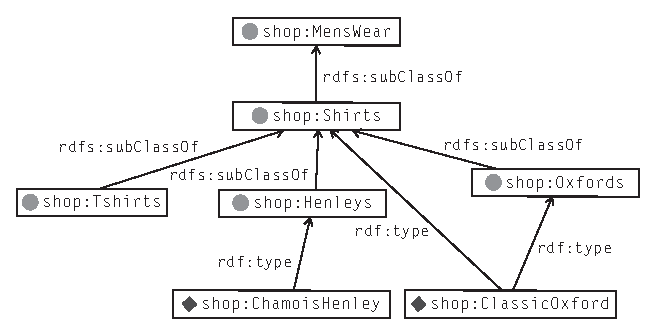
\includegraphics[width=5in]{media/ch7/f07-02.eps}
\caption{Asserted triples in the catalog model.}
\label{fig:ch7.2}
\end{figure}

An inferencing query engine that enforces just the type propagation rule
will draw the following inferences (for the purpose of these examples, an asterisk denotes an inferred triple):

\begin{lstlisting}
*shop:ChamoisHenley rdf:type shop:Shirts .
*shop:ChamoisHenley rdf:type shop:MensWear .
*hop:ClassicOxford rdf:type shop:Shirts .
*shop:ClassicOxford rdf:type shop:MensWear .
*hop:BikerT rdf:type shop:Shirts .
*shop:BikerT rdf:type shop:MensWear .
\end{lstlisting}

\begin{figure}
\centering
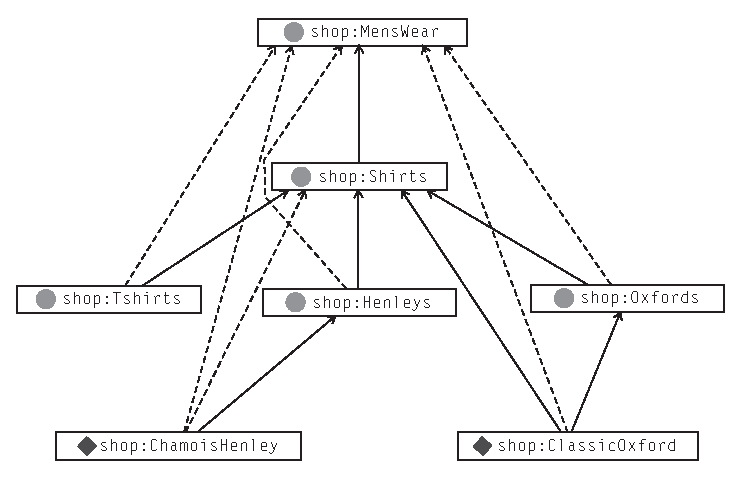
\includegraphics[width=5in]{media/ch7/f07-03.eps}
\caption{All triples in the catalog model. Inferred triples are shown as dashed
lines.}
\label{fig:ch7.3}
\end{figure}



Some of these triples were also asserted; the complete set of triples
over which queries will take place is as follows, with inferred triples
in italics:

\begin{lstlisting}
shop:Henleys rdfs:subClassOf shop:Shirts.
shop:Shirts rdfs:subClassOf shop:MensWear.
shop:Blouses rdfs:subClassOf shop:WomensWear.
shop:Oxfords rdfs:subClassOf shop:Shirts.
shop:TShirts rdfs:subClassOf shop:Shirts.
shop:ChamoisHenley rdf:type shop:Henleys.
*shop:ChamoisHenley rdf:type shop:Shirts.
*shop:ChamoisHenley rdf:type shop:MensWear.
shop:ClassicOxford rdf:type shop:Oxfords.
shop:ClassicOxford rdf:type shop:Shirts.
*shop:ClassicOxford rdf:type shop:MensWear.
shop:BikerT rdf:type shop:Tshirts.
*shop:BikerT rdf:type shop:Shirts.
shop:BikerT rdf:type shop:MensWear.
\end{lstlisting}

All triples in the model, both asserted and inferred, are shown in
Figure\ref{fig:ch7.3}. We use the convention that asserted triples are printed with
unbroken lines, and inferred triples are printed with dashed lines. This
convention is used throughout the book.
\end{example}

The situation can become a bit more subtle when we begin to merge
information from multiple sources in which each source itself is a
system that includes an inference engine. Most RDF implementations
provide a capability by which new triples can be asserted directly in
the triple store. This makes it quite straightforward for an application
to assert any or all inferred triples. If those triples are then
serialized (say, in RDF/XML) and shared on the Web, another application
could merge them with other sources and draw further inferences. In
complex situations like this, the simple distinction of asserted versus
inferred might be too coarse to be a useful description of what is
happening in the system.

\section{When Does Inferencing Happen?}

The RDFS and OWL standards define what inferences are valid, given
certain patterns of triples. But when does inferencing happen? Is
inferencing done at all? Where and how are inferred triples stored, if
at all? How many of them are there?

These questions are properly outside the range of the definitions of
RDFS and OWL, but they are clearly important for any implementation that
conforms to these standards. It should, therefore, come as no surprise
that the answers to these questions can differ from one implementation
to another. The simplest approach is to store all triples in a single
store, regardless of whether they are asserted or inferred. As soon as a
pattern is identified, any inferred triples are inserted into the store.
We will call this \emph{cached inferencing}, since all inferences are
stored (``cached'') with the data. This approach is quite simple to
describe and implement but risks an explosion of triples in the triple
store. At the other extreme, an implementation could instead never
actually store any inferred triples in any persistent store at all.
Inferencing is done in response to queries only. We will call this
\emph{just in time inferencing}, since the inferences are computed at
the latest possible moment. The query responses are produced in such a
way as to respect all the appropriate inferences, but no inferred triple
is retained. This method risks duplicating inference work, but it is
parsimonious in terms of persistent storage. These different approaches
have an important impact in terms of change management. What happens if
a data source changes---that is, a new triple is added to some data
store or a triple is removed? A strategy that persistently saves
inferences will have to decide which inferred triples must also be
removed. This presents a difficult problem, since it is possible that
there could be many ways for a triple to be inferred. Just because one
inference has been undermined by the removal of a triple, does that mean
that it is appropriate to remove that triple? An approach that
recomputes all inferences whenever a query is made need not face this
issue.

An important variant of just in time inferencing is where no explicit
inferencing is done at all. We already saw, in our example about
subclasses of Shirts, how a query could explicitly express what data it
wanted, without relying on the inference semantics of the model at all.
As we see in the next section, even in this case, where there is no
explicit inferencing, the inference interpretation of a model is still
important in organizing and understanding a semantic application.

\subsection{Inferencing as specification}

At the beginning of this chapter, we looked at a query to find all the
Shirts in a catalog, explicitly tracing down the all rdfs:subClassOf
links:

\begin{lstlisting}
SELECT ?item
WHERE {?class rdfs:subClassOf* :Shirts .
?item a ?class . }
\end{lstlisting}

This selection was done to support a search operation---``find me all
the Shirts.'' This query operates without any explicit reference to
inference at all; it returns its answers without reference to inferred
triples vs. asserted triples; it just processes the asserted data. But
how do we know that the items returned by this query are Shirts?

This same question could be asked of a program in Java or C++ or even
SQL---if we write a program to collect up the members of all the
subclasses of Shirts (and their subclasses, and so on), do we know that
all the things we have collected are Shirts? If we return one of these
things as the result of a user search, can we be justified in thinking
that it is itself a shirt? This suggests a role that a semantic model
can play in the interpretation of data---it can tell us whether the
queries we have written are correct. In this example, our model tells us
that every Henley is a shirt, because the class Henleys is a subclass of
the class Shirts. The same goes for Oxfords, and for any subclasses of
Oxfords. The model, along with its formal semantics, guarantees that all
the results of this query will indeed be shirts.

In this sense, the model is a specification. Any discussion about the
appropriateness of a particular query can appeal to the model for
arbitration---is this query consistent with the model? In this example,
the model tells us that any result from this query will be a Shirt, so
it is appropriate to treat them as such. When the model is written in a
language for which there is a capability to do automated inferences
(like RDFS, RDFS-Plus, or OWL), it becomes particularly useful---the
specification is said to be executable. This means that we can run a
program that will tell us exactly what the model means. In the example
above where we showed asserted and inferred triples, we showed the
results of just such a capability, resulting in a list of all the Shirts
(of any type).

When building an application, we might decide to use a general-purpose
inference capability, or we might decide to use an extended query (like
the one shown here), or we might write a program in some other language.
A specification (even an executable one) tells us what our program or
query ought to do; it doesn't tell us how we should do it. Regardless of
this implementation choice, the model plays a central role of justifying
the query or program. If many people develop different systems (even
using different technological approaches), the results they provide will
be consistent, if they justify them all against the same model.


\section{Expectation in RDF}


In Chapter~\ref{ch1}, we examined some of the assumptions around managing information on the web, 
whether it is to be consumed directly by humans or first by machines.  One of the basic assumptions is
that we cannot know, in advance, what we will find on the web, therefore, we must proceed with the \emph{Open World} assumption (Section~\ref{openworld}).  We only draw conclusions from data that will not be undermined or countermanded by the discovery of new data.  This assumption makes sense when we are interpreting data we find in the wild.

But there are some situations in which we are not interpreting data, we instead are acting on some expectations about the
data in the wild.  Our expectations about data might come from regulatory control (an application for a loan must
include certain information about the borrower), or our own business policies (we require certain information about a
prospective borrower before we will consider a loan), or just plain common sense (a borrow's date of birth cannot be in
the future).

Expectations in the Semantic Web can take three broad forms:

\begin{itemize}
    \item \emph{Data Validation} \label{datav} Data found in the wild purports to describe a particular kind of thing, and we have
    expectations about that type.  We want to validate that the data matches our expectations.

  \item \emph{Soliciting user input} \label{form}
      We might not find our data published on the web as a linked data resource, but
      rather, we want to request input from a user.  In this case, we want to be able to communicate to that user what
      our expectations are for the data they will provide.  This is typically done with a form or a wizard that a user
      fills out with the data they are providing.

    \item \emph{Validating user input} \label{userv} Even when we have communicated our expectations to a user,
      they might not provide 
      data in the form we expect.  In this case, just as in the first case, we will want to validate our data against our
      expectations.
\end{itemize}

We can think of our expectations for a data description as a specification of the \emph{shape} that the data should take.  This metaphor is quite literal in case \ref{form} above, where the expected shape of the data is presented in a form that a user will fill out.  

Beyond the shape of a data description, our expectations can also place constraints on values.  The age of an adult must be greater than 18 (or 21, depending on the intent of the data shape in question);  a social security number must be of the form XXX-XX-XXXX.

These intuitions are the motivation behing the name of the expectation modeling language of the Semantic Web, \emph{SHACL}, Shapes Constraint Language.  SHACL provides a mechanism for specifying the expected shape of a data description and constraints on its validity.

We'll illustrate all three uses of SHACL with a single example, shown in Figure~\ref{fig:ch7.account}.

\begin{figure}
  \begin{lstlisting}
 1. @prefix sh: <http://www.w3.org/ns/shacl#> .
 2. account:Account
 3.   rdf:type sh:NodeShape ;
 4.   rdfs:label "Account" ;
 5.   sh:property [
 6.       rdf:type sh:PropertyShape ;
 7.       sh:path account:lastName ;
 8.       sh:datatype xsd:string ;
 9.       sh:name "family name" ;
10.       sh:description "the name shared by all members of a family" ;
11.       sh:maxCount 1 ] ;
12.   sh:property [
13.       rdf:type sh:PropertyShape ;
14.       sh:path account:ssn ;
15.       sh:datatype xsd:string ;
16.       sh:description
17.            "US Social Security Number - format XXX-XX-XXXX" ;
18.       sh:maxCount 1 ;
19.       sh:minCount 1 ;
20.       sh:name "SSN" ;
21.       sh:pattern
22.          "[0-9][0-9][0-9]-[0-9][0-9]-[0-9][0-9][0-9][0-9]" ] ;
23.   sh:property [
24.       sh:path account:gender ;
25.       sh:datatype xsd:string ;
26.       sh:in (
27.           "female"
28.           "male"
29.         ) ;
30.       sh:maxCount 1 ;
31.       sh:name "gender" ] .
  \end{lstlisting}
  \caption{Listing of a SHACL model for an Account}
  \label{fig:ch7.account}
\end{figure}

The first thing to notice about Figure~\ref{fig:ch7.account} is that it is expressed in RDF.  This is typical of the langauges of the Semantic Web; every language is expressed in RDF, so that the models in that language can be distirbuted across the web as linked data sets in their own right (see Chapter~\ref{ch5}. 

The second thing to notice is the large number of resources whose names
begin with \texttt{sh:}.  As we see in line 1, this is a prefix abbreviation for
\texttt{http://www.w3.org/ns/shacl\#}, which is a domain prefix controlled by the
W3C (as we saw in Section~\ref{minting-http-uris}).  This is also typical of how a
new language is built on top of RDF; the language publisher (in this case, the W3C)
defines a number of resources in a single domain that they control.  If you dereference
one of these HTTP URIs, the result (which is maintained by the same publisher, the W3C) is a 
description of that resource.  If you paste the HTTP URI 
\texttt{http://www.w3.org/ns/shacl\#} into a web browser, you will see the W3C 
Recommendation document that describes SHACL.


Now let's dive into the details of the shapes.  
In the data, we have three entities that claim to be \texttt{Accounts}.  For
each of them, certain data is provided; first names, last names, SSN, gender.
The shapes in Figure~\ref{fig:ch7.account} specifies our expectations about these
things.

There are three constraints on properties defined in Figure~\ref{fig:ch7.account}, beginning on lines 5, 12 and 23.  The property that they place a constraint on is given by \texttt{sh:path}, so they constrain \texttt{account:lastName} (line 7), \texttt{account:ssn} (ine 14)  and \texttt{account:gender} (line 24) respectively.

Each of these constraints say something different about the property.  
In the case of \texttt{account:lastName} (lines 5-11), the constraint says 
that the value must be a string,  and that there can be at most one value.

In the case of \texttt{account:ssn} (lines 12-22), there must be exactly one value 
(both min and max of 1 are specified), it must be a string, but it also must match
a pattern given by a regular expression.  Regular expressions are beyond the scope
of this book, but this one says that the string must have the form ``XXX-XX-XXXX''
where each X is a digit from 0 to 9.

Finally, the third contraint, on \texttt{account:gender} (lines 23-31) specifies that
there can be at most one value, and that value must be in the list given, that is, one
of ``male'' or ``female''.

\hypertarget{validating-data}{%
\subsection{Validating data}\label{validating-data}}


Let's see how this works, first in the context
of data validation.  Suppose we have data about the active accounts as shown in
Figure~\ref{fig:ch7.data}.


\begin{figure}
  \begin{lstlisting}
active:Account_1
  rdf:type account:Account ;
  rdfs:label "Account 1" ;
  account:firstName "Aaron" ;
  account:gender "male" ;
  account:lastName "Beatte" ;
  account:ssn "123-45-6789" .

active:Account_2
  rdf:type account:Account ;
  rdfs:label "Account 2" ;
  account:firstName "George" ;
  account:gender "unknown" ;
  account:lastName "Deller" ;
  account:ssn "12-345678" .

active:Account_3
  rdf:type account:Account ;
  rdfs:label "Account 3" ;
  account:firstName "Edelyn" ;
  account:lastName "Zetta" .
  \end{lstlisting}
\label{fig:ch7.data}
\caption{Data to be vaidated by Figure~\protect\ref{fig:ch7.account}.}
\end{figure}

First off, each descriptions in Figure~\ref{fig:ch7.data} has a single string value for
\texttt{account:lastName}, as expected.  So there is no violation in this data set for \texttt{lastName}.

Now let's look at \texttt{account:gender}.  \texttt{Account\_1} has the
value ``male'', which is one of the expected values, so there is no
violation.  \texttt{Account\_2} has the value ``unknown'' for \texttt{account:gender}.  This is not one 
of the expected values, so this is a violation.  SHACL can be quite specific about
the violation - the given value, ``unknown'', is not in the list of allowed
values (``female'', ``male'').  \texttt{Account\_3}, on the other hand, has 
no value at all for \texttt{account:gender}.  The constraint says that the
maximum number of values we can have for this property is 1, but says nothing about the
minimum number of values.  So, according to this shape, the correct way to specify
an unknown gender (or an unwillingness to provide one from the list ``male''
and ``female'') is to leave it out. 

The constraint on \texttt{account:ssn} specifies a pattern that a SSN should take.
In our data, \texttt{active:Account\_1} specifies a SSN of the appropriate format.
\texttt{active:Account\_2} specifies an SSN, but the format does not match.  SHACL can
be very specific about the violation, that the value for \texttt{account:ssn}
does not match the pattern given in the shape.  Finally, \texttt{active:Account\_3}  provides no value for SSN at all.  In this case, the shape specifies (line 18, Figure~\ref{fig:ch7.account}) \texttt{sh:minCount 1}, so, unlike the case of the missing
gender, this is a violation, namely, property needs at least 1 value, found 0.

The process we just outlined is called \emph{SHACL validation}; given a set of
shape defintions in SHACL, and data that purports to conform to those shapes,
we can automatically determine whether and how the data violates the constraints
given in the shape.

Validation is important in the web of data, since the applications
that publish and consume data from the Web of data are  written and
hosted by different organizations.  if we want to ensure
interoperability between open and heterogeneous systems, we need a way
to specify our expectations about the data they will provide and
consume.  SHACL provides a way to specify those expectations, and
SHACL validation provides a way to enforce them.



\subsection{Soliciting User Input}\label{soliciting}

The same constraints that allow us to validate data can be used to
control the solicitation of data from a user.  Take the shape given in
Figure~\ref{fig:ch7.account}.  Just intuitively, if we wanted to make
a form for a user to fill out, we would expect the form to have three
fields, one each for \texttt{account:lastName}, \texttt{account:ssn}
and \texttt{account:gender}.  But we of course don't expect a form to
use the QName of a property to elicit input.  Fortunatlely,
Figure~\ref{fig:ch7.account} also provides names for each of the
constraints, and these names are more suitable for human consumption;
``family name'', ``SSN'' and ``gender''.  If further information is
needed about any of these things (e.g., what does SSN stand for?),
there is the \texttt{sh:description}, which describes it in more
detail.  In the case of \texttt{account:gender}, the constraint even
provides a suggestion for how the form should operate; it should only
provide two options for the answer, corresponding to the two
accpetable answers, ``male'' and ``female''.

There are any number of technologies avaiable for producing forms for
people to fill in; SHACL simply provides the content, in terms of
field names, types, and allowable values that the forms should have.
Figure~\ref{fig.ch7.form} shows an example form created from the shape
in Figure~\ref{fig.ch7.account}, using basic HTML.



\subsection{Validating User Input}\label{vuser}

One of the advantages of using a machine-readable shapes language like
SHACL (remember, SHACL is in RDF, so we can query over it using
SPARQL, as we saw in Chapter~\ref{ch6}) is that we can use the same
model (Figure~\ref{fig.ch7.account}) to drive data validation
(Section~\ref{validating-data}) as we use to solicit data from human
users (Section~\ref{soliciting}).  We can combine these processes, and
use the same model to validate user input.

We've already seen that the model can be used to prevent certain data
errors by users.  By buiding a form that only accepts values ``male''
and ``female'', we prevent a user from submitting a form with a value
like ``unknown''.  But, depending on the technology we are using for
the forms, we might not be able to enforce all of the constraints
expressed in a shape with a form.

For example, the constraint on SSN is somewhat elaborate; it requires
something that can check a regular expression against the human
input.  Simple HTML forms don't have a facility for regular
expressions, so we just have to leave it to the human to fill in the
form, and hope that they follow the format suggestion given in the
\texttt{sh:description} field of the shape.

Once we have the results from the form, we can process it using the
same tool that we used for data on the web, namely, a SHACL
validator. This allows us to make sure that the data entered by a
human user will conform to the same high standard as data we find on
the web.

In this way, SHACL helps us to retain the value of the data wilderness
while, to some extent, taming its wild nature.  We still accept data
from across the web, we still allow anyone to say anything about any
topic, but we protect our data applications from runaway behavior by
enforcing shapes and constraints on the data.


\section{SUMMARY}

RDF provides a way to represent data so that information from multiple
sources can be brought together and treated as if they came from a
single source. But when we want to use that data, the differences in
those sources comes out. For instance, we'd like to be able to write a
single query that can fetch related data from all the integrated data
sources.

The Semantic Web provides an approach to this problem in the form of
modeling languages in which the relationship between data sources can be
described. A modeling construct's meaning is given by the pattern of
inferences that can be drawn from it. Information integration can be
achieved by invoking inferencing before or during the query process; a
query returns not only the asserted data but also inferred information.
This inferred information can draw on more than one data source.

We have seen how even very simple inferencing can provide value for data
integration. But just exactly what kind of inferencing is needed? There
isn't a single universal answer to this question. The

Semantic Web standards identify a number of different levels of
expressivity, each supporting different inferences, and intended for
different levels of sophistication of data integration over the Semantic
Web.

In the following chapters, we will explore three particular inferencing
levels. They differ only in terms of the inferences that each of the
languages allow. RDFS (Chapter 6) is a recommendation defined and
maintained by the W3C. It operates on a small number of inference rules
that deal mostly with relating classes to subclasses and properties to
classes. RDFS-PLUS (Chapter 7) is a mode that we have defined for this
book. We have found a particular set of inference patterns to be helpful
both pedagogically (as a gentle introduction to the more complex
inference patterns of OWL) and practically (as a useful integration tool
in its own right). RDFS-PLUS builds on top of RDFS to include
constraints on properties and notions of equality. OWL (Chapters 9 and
10) is a recommendation defined and maintained by the W3C, which builds
further to include rules for describing classes based on allowed values
for properties. All of these standards use the notion of inferencing to
describe the meaning of a model; they differ in the inferencing that
they support.

\subsection{Fundamental concepts}

The following fundamental concepts were introduced in this chapter.

\begin{itemize}
\item Inferencing---The process by which new triples are systematically added
to a graph based on patterns in existing triples.

\item Asserted triples---The triples in a graph that were provided by some
data source.

\item Inferred triples---Triples that were added to a model based on
systematic inference patterns.

\item Inference rules---Systematic patterns defining which of the triples
should be inferred.

\item Inference engine---A program that performs inferences according to some
inference rules. It is often integrated with a query engine.

\item
  SHACL shapes to validate RDF data at the structural level by providing
  the constraint you expect them to meet.
  \end{itemize}
  
